\section{Retrieving and displaying results} \label{disp_results}

To get at the results, we can query the tree or the initializer and/or optimizer returned by \\
\texttt{[initializer, optimzer] = tree.solve()}.
Some examples:

\begin{verbatim}
tree.plotTree();
\end{verbatim}

This displays a pictoral representation of the tree structure--useful for double-checking
if your input is what you thought it was.
See Figure \ref{fig:tree_example} for an example of output.

\begin{figure}[t]
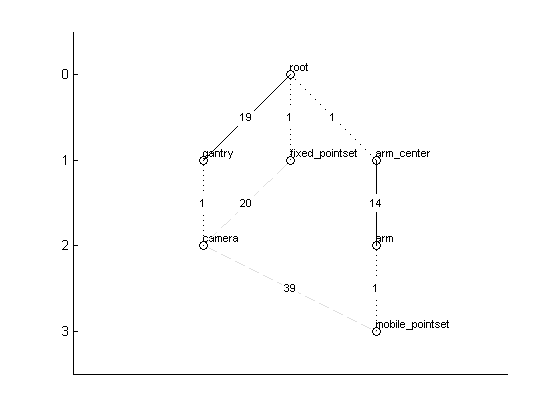
\includegraphics{figures/tree_example}
\caption{Example output for \texttt{tree.plotTree()}.}
\label{fig:tree_example}
\end{figure}

\begin{verbatim}
[x,resnorm,residual,exitflag,output,lambda,jacobian] = optimizer.lsqnonlinReturnValues{:};
\end{verbatim}

Caliber uses \texttt{lsqnonlin} internally; it stores the return values of that function in \texttt{optimizer.lsqnonlinReturnValues}.

\begin{verbatim}
optimizer.printSolutionInfo();
\end{verbatim}

This prints out information on the solution found by Caliber--all tweaks and their corresponding data values. An example:

\small
\begin{verbatim}
camera1           K          7051         <fixed>        700.6      
                            <fixed>        7052          471.8      
                            <fixed>       <fixed>       <fixed>     

camera1           kc        -0.08879    
                            -11.95      

camera2           K          3488         <fixed>        689.6      
                            <fixed>        3488          477.6      
                            <fixed>       <fixed>       <fixed>
...
\end{verbatim}
\normalsize

\begin{verbatim}
tree.plotPixelErrors();
\end{verbatim}

\begin{figure}[t]
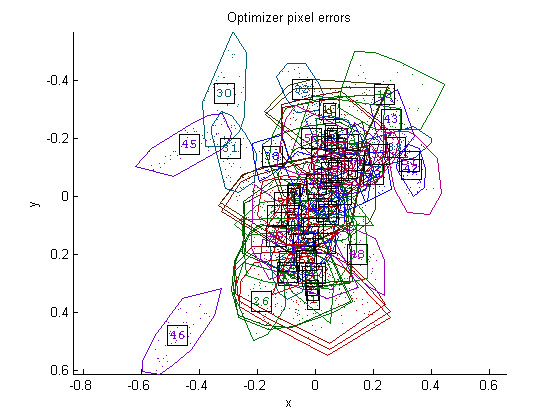
\includegraphics{figures/pixel_example}
\caption{Example output for \texttt{plotPixelErrors()}.}
\label{fig:pixel_example}
\end{figure}

This plots all reprojection errors, similar to Bouguet's \textsf{Analyse error} button.
Points are plotted as single pixels; the pixels for each observation get a single color,
a convex hull, and a label with the observation number at the centroid.
See Figure \ref{fig:pixel_example} for an example of output.

\begin{verbatim}
tree.plotExtrinsics();
\end{verbatim}

\begin{figure}[t]
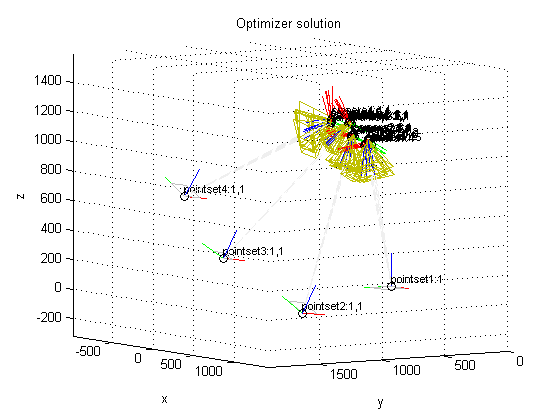
\includegraphics{figures/extrinsic_example}
\caption{Example output for \texttt{plotExtrinsics()}.}
\label{fig:extrinsic_example}
\end{figure}

This makes a 3-D plot (in the root frame) of camera and pointset transformations for each observation,
somewhat similar to Bouguet's \textsf{Show extrinsic} button, but accounting for 
the fact that there may be multiple cameras and/or pointsets.
See Figure \ref{fig:extrinsic_example} for an example of output.

\begin{verbatim}
tree.plotImagePoints();
\end{verbatim}

\begin{figure}[t]
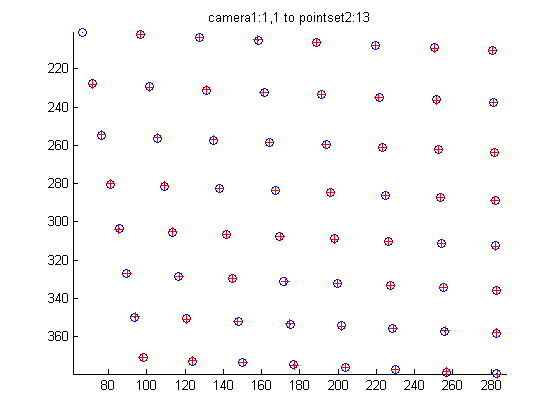
\includegraphics{figures/image_example}
\caption{Example output for \texttt{plotImagePoints()}.}
\label{fig:image_example}
\end{figure}

This makes one plot per observation of the observed image points and the reprojections of the solution.
See Figure \ref{fig:image_example} for an example of output. Note that the plots depend on the specific
observation types.

\begin{verbatim}
tree.relativeM('camera', Map({'main_arm', 'lamp_arm'}, {1, 2}), 'lamp_pointset');
\end{verbatim}

For the spherical gantry case, this gets the relative transformation between the camera and the lamp pointset 
when the main arm is in state 1 and the lamp arm is in state 2. You can specify a different set of node states for the pointset
with a fourth argument.

